\FloatBarrier
\subsection{Infrastructure realization}
\subsubsection{Infrastructure overview}
Einstein Telescope will have excellent sensitivity of about $10^{-22}/\sqrt{\mathrm{Hz}}$ at low frequency (2\,Hz). This is achieved by employing advanced suspension systems, discussed in Chapter \ref{sec:suspension_systems}, with a frequency cut-off below 1.8\,Hz at a site that features low seismic noise. Fig.~\ref{fig:sitecomparison} shows that various excellent candidate sites for Einstein Telescope have been identified in Europe. Einstein Telescope will be constructed underground in order to benefit from low seismic and gravity gradient noise. It is well known that the major part of the seismic noise in the frequency range 1 to 10\,Hz is generated at the surface. The corresponding gravity gradient noise is then partly suppressed at underground locations due to surface averaging effects. The gravity gradient noise attenuation factor has been shown in Fig.~\ref{fig3.8}. It is seen that gravity gradient noise effects from surface waves can be attenuated by more than 2 orders of magnitude for frequencies $f > 2$\,Hz for underground detectors at moderate depth ($>100$ m) for soft-soil and homogeneous conditions. Dedicated studies~\cite{GGCellaCuoco} show that in general it will be a challenge to obtain sites with low gravity gradient noise properties. Finite element analysis calculations reveal large differences in attenuation between 1 and 2 Hz. The required depth is driven partly by the wavelength of the seismic waves. Roughly $\lambda / 4$ is required for about a factor of 100 suppression. The wavelength scales with the seismic velocity. While for soft soil typical values of 440\,m/s are found for the longitudinal velocity $c_L$, these values increase to 6000\,m/s for stressed hard rock such as granite at great depth. Consequently, while the depth of Einstein Telescope could be limited to a few hundred meters when constructed in soft soil, significantly larger depths may be required when considering siting in hard rock. 
\begin{figure}[htbp!]
	\centering
		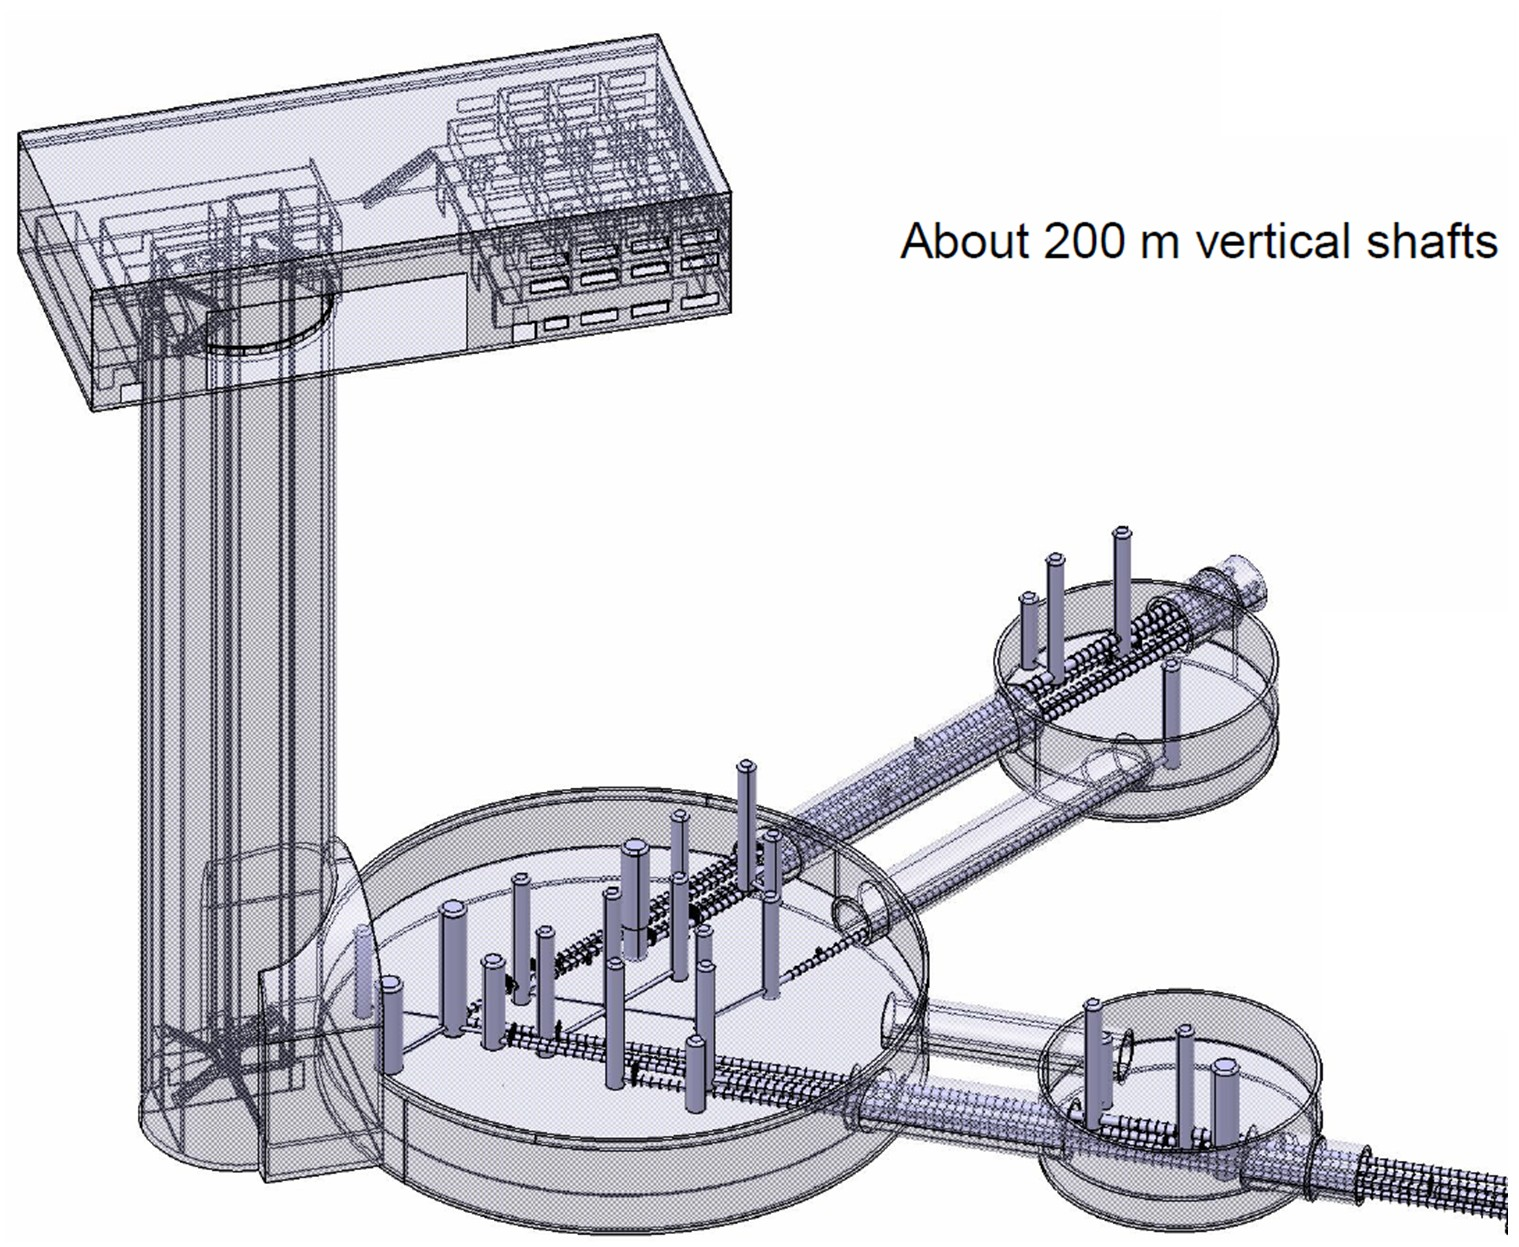
\includegraphics[width=10cm]{./Sec_SiteInfra/Figures/infra.jpg}
		\caption{Impression of one of the corner stations for Einstein Telescope. Surface buildings connect via a vertical shaft to the underground facilities that feature one main cavern and two satellite caverns. The observatory has a triangular configuration that can house three xylophone detectors. Each detector is composed of a low-frequency cryogenic interferometer and a high-frequency interferometer operated at room temperature. The three corner stations are connected by 10 km long tunnels.}
		\label{fig:infra}
\end{figure}

The Einstein Telescope site studies were performed at various underground locations in hard rock (Frejus, Canfranc, Gran Sasso, Sardinia and Hungary in Europe, Homestake in the USA, and Kamioka in Japan), in salt (Slanic Salt Mine in Romenia, and Realmonte in Sicily), and in Boom clay (the HADES facility for storage of nuclear waste in Mol, Belgium). The lowest seismic noise was obtained in hardrock. Note that homogeneity and seismic correlation length of the medium are expected to be important parameters for future gravity gradient noise subtraction schemes.

The realization of Einstein Telescope requires the construction of substantial underground infrastructure. Fig.~\ref{fig:infra} shows an impression of the one of the corner stations of the observatory.
\begin{figure}[htbp!]
\centering
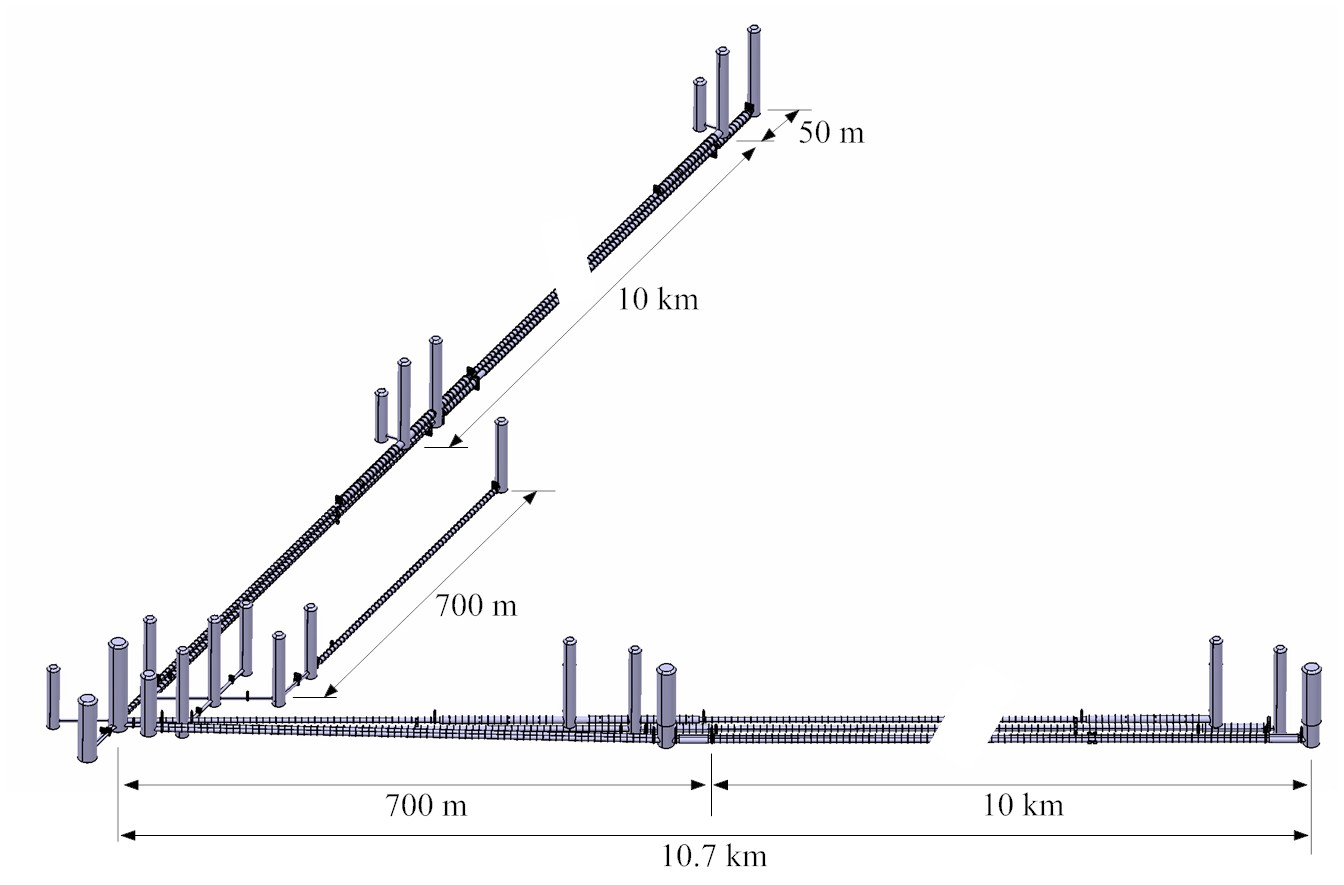
\includegraphics[width=14cm]{./Sec_SiteInfra/Figures/infra2.jpg}
\caption{Global view of a single xylophone detector showing the vacuum system and suspension towers needed to house the various optical components. Note that distances are not to scale.}
\label{fig:infra2}
\end{figure}

\begin{figure}[htbp!]
\centering
\includegraphics[width=11cm]{./Sec_SiteInfra/Figures/infra7.jpg}
\caption{Global layout of Einstein Telescope. Upper panel: during phase I the observatory will house a single xylophone detector. Lower panel: in phase II a triple xyolophone detector system will be implemented. Note that distances are not to scale.}
\label{fig:infra1}
\end{figure}
The Einstein Telescope observatory has a triangular topology that houses up to three xylophone detectors. The first phase of the project features a single xylophone configuration that consists of a cryogenic low-frequency interferometer and a room-temperature high-frequency  interferometer (see Fig.~\ref{fig:infra1}).

The three corner stations are connected by 10 km long tunnels. Each corner station consists of a collection of surface buildings. The main assembly building gives access to a 20 m diameter shaft that leads to the underground infrastructure. At each corner there are three large experimental caverns, the main cavern houses the laser injection systems and the beam splitters, while both the end-test masses of the filter cavities for the high frequency beams (ETM-FC-HF) and the input test masses of the filter cavities for the low frequency beams (ITM-FC-LF) occupy the auxilliary caverns. Tunnels house the interferometer arms and have an inner diameter of 5.5 m. In the following we discuss infrastructure aspects of the tunnels, underground caverns, and the vertical shafts and their construction. In addition, we discuss issues encountered at other underground projects and that may be of relevance for Einstein Telescope.

\FloatBarrier
\subsubsection{Caverns}
\label{subsec:caverns}
\subsubsection*{Main caverns}

\begin{figure}[htbp!]
\centering
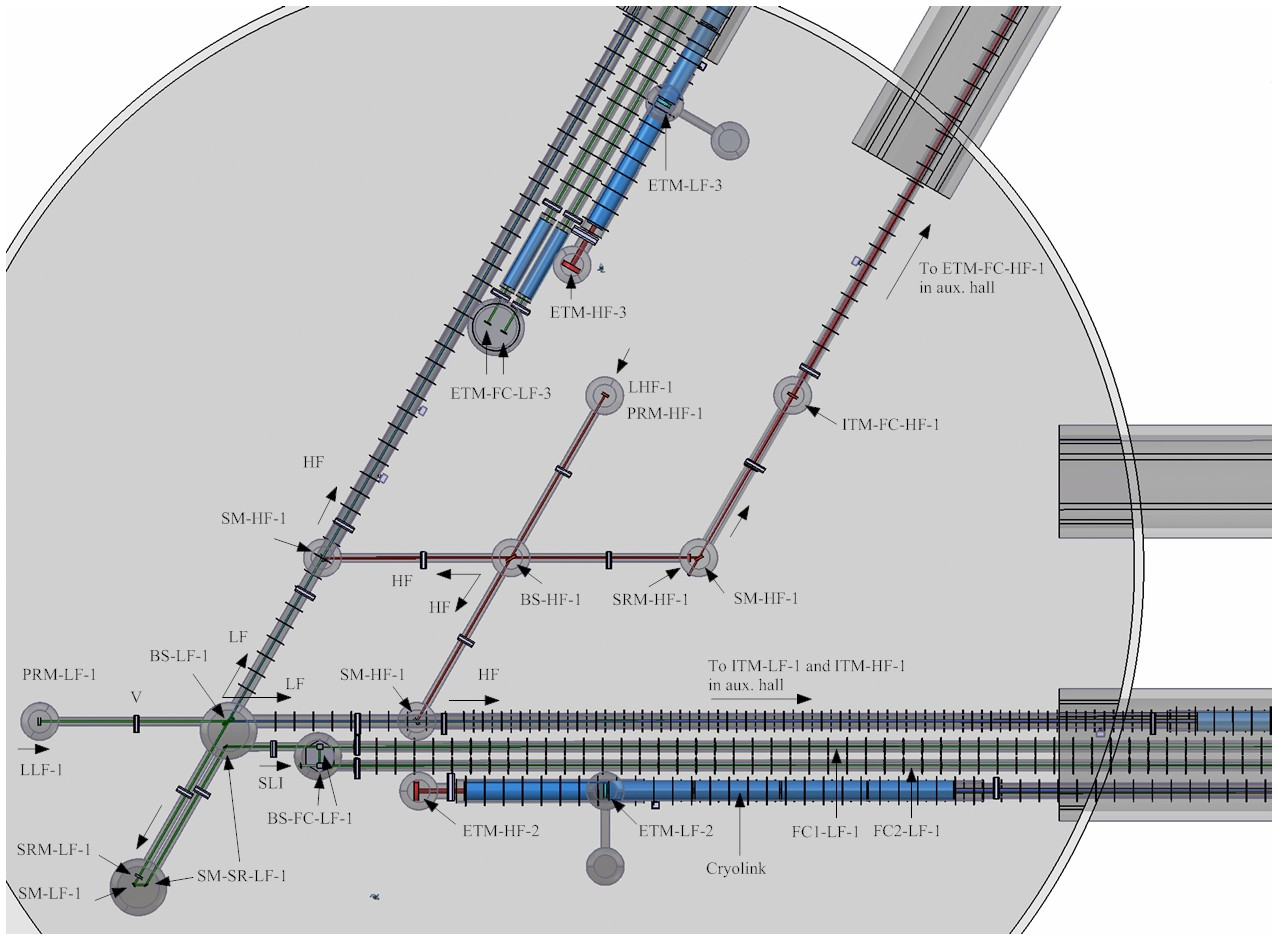
\includegraphics[width=22.5cm, angle=90]{./Sec_SiteInfra/Figures/infra3.jpg}
\caption{Schematic outline of the main infrastructure in one of the large underground caverns.
The labels are explained in the text.}
\label{fig:infra3}
\end{figure}
An outline of the detector system in one of the large underground caverns is shown in Fig.~\ref{fig:infra3}. The cavern has a cylindrical shape with 65 m diameter and 30 m height. It contains detector components from all three xylophones (denoted by the last number on the labels). The laser of the low-frequency interferometer for xylophone 1 is denoted LLF-1. It injects into the power-recyling mirror PRM-LF-1 and is directed onto beamsplitter BS-LF-1. Arrows indicate the directions of the two beams towards the 10 km long interferometer arms. In the same manner the laser of the high-frequency beam of xylophone detector 1 is denoted LHF-1. It injects the beam into PRM-HF-1 and then onto beamsplitter BS-HF-1. Again arrows indicate the directions of the two beams. Steering mirrors, SM-HF-1, are used to direct both HF beams towards the long interferometer arms. Steering mirrors are used solely in the HF beams, since the requirements for low-frequency seismic noise isolation are less stringent for HF beams than for the LF beams. Both LF and HF beams use separate beam pipes. The LF beam is on top (in the vertical direction) of the HF beam as this approach simplifies the cryogenic superattenuator design (see section 3.8).

The LF beam at the dark port ends on signal-recycling mirror SRM-LF-1. The light is bounced off three steering mirrors, indicated in Fig.~\ref{fig:infra3} by SM-SR-LF-1, and is directed towards a beamsplitter at the entrance of filter cavity 1, BS-FC-LF1. Part of the light now enters the beam tube of filter cavity 1, FC-1-LF-1, and falls on the injection test mass ITM-FC2-LF-1 located in the auxilliary cavern. FC-1-LF-1 is 10 km long and ends on the end test mass ETM-FC-LF-1 located in the main underground cavern at the other side of the interferometer arm. The other part of the light enters a second filter cavity, FC-2-LF-1, and via ITM-FC-2-LF-1 in the satellite cavern it enters the 10 km long filter cavity. Again a test mass is located in the corner station at the other end. Both filter cavities use separate beam pipes. The low frequency interferometer allows injection of squeezed light (indicated in Fig.~\ref{fig:infra3} with label SLI). 

Also the HF beam at the dark port implements a filter cavity. Light from signal recycling mirror SRM-HF-1 is reflected via steering mirror SM-R-HF-1 into the injection test mass ITM-FC-HF-1 of the filter cavity. The cavity is 300 m long and the end test mass ETM-FC-HF-1 is located in an satellite cavern.

Each main underground cavern houses two end test masses of both other interferometers. In Fig.~\ref{fig:infra3} this is indicated by ETM-LF-2 and ETM-LF-3 for the two other low-frequency interferometers, and by ETM-HF-2 and ETM-HF-3 for the other high-frequency interferometers. In addition, the main cavern houses the two end test masses of the filter cavities for one of the other low-frequency interferometers. In Fig.~\ref{fig:infra3} this is indicated with ETM-FC-LF-3.

The main optical components of the interferometers need to be suspended. Each main cavern houses 17 suspension towers; 4 of these towers are part of the cryogenic suspension system needed for the suspension of the end test masses of the two other LF interferometers. Three towers are used to suspend double payloads, while three towers are used to suspend triple payloads. In two cases the low frequency beam passes through the suspension system of the high frequency beam. 

The main cavern is occupied by two cryolinks that protect the cryogenic end test masses of both other interferometers from thermal radiation. In addition, cryolinks are employed near the end test masses of the filter cavity of one of the other interferometers. The cavern must accommodate the cryogenic infrastructure needed for the operation of the four cryolinks.

It can be seen in Fig.~\ref{fig:infra3} that each main cavern is connected to four tunnels. Two of these tunnels accommodate six vacuum beam pipes, a third tunnel holds the filter cavity for the high frequency interferometer, and the fourth tunnel is empty. The latter is used to allow transportation xof equipment between main cavern and satellite cavern.

\FloatBarrier
\subsubsection*{Satellite caverns}

\begin{figure}[htbp!]
\centering
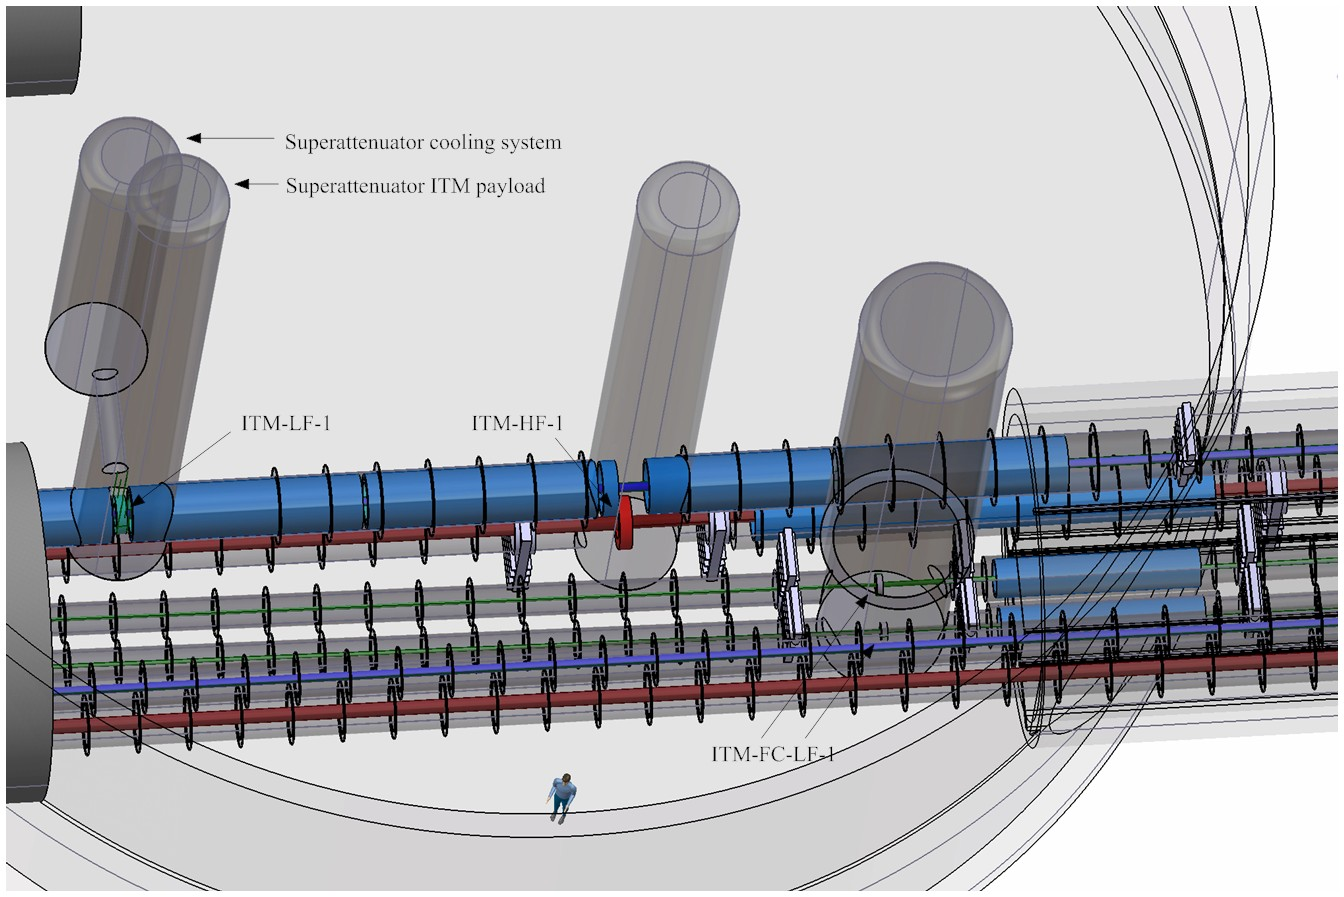
\includegraphics[width=16cm]{./Sec_SiteInfra/Figures/infra4.jpg}
\caption{Schematic outline of the main infrastructure in one of the satellite underground caverns.
The labels are explained in the text.}
\label{fig:infra4}
\end{figure}

An impression of the infrastructure of one of the satellite caverns is shown in Fig.~\ref{fig:infra4}. The necessity of having these satellite caverns is explained in Chapter 5. These caverns are cylindrical in shape with a diameter of 30 m and a height of 30 m. In its final configuration, six beam pipes pass through this cavern. The cavern is occupied by the input test masses of both the low frequency and high frequency interferometer. The low frequency ITM is a cryogenic payload and is surrounded with a cryolink. The cavern is equipped with the necessary cryogenic infrastructure. It can be seen in Fig.~\ref{fig:infra3} that each satellite cavern provides the entrance to a main interferometer arm tunnel.

\FloatBarrier
\subsubsection*{Cavern construction issues}

Einstein Telescope will have a total of 9 underground caverns. Each corner station
will have a large cylindrical underground cavern with a diameter of about 65 m and a
height of 30 m. Each corner station will have two smaller satellite caverns
with diameter and height of 30 m.

\begin{figure}[htbp!]
\centering
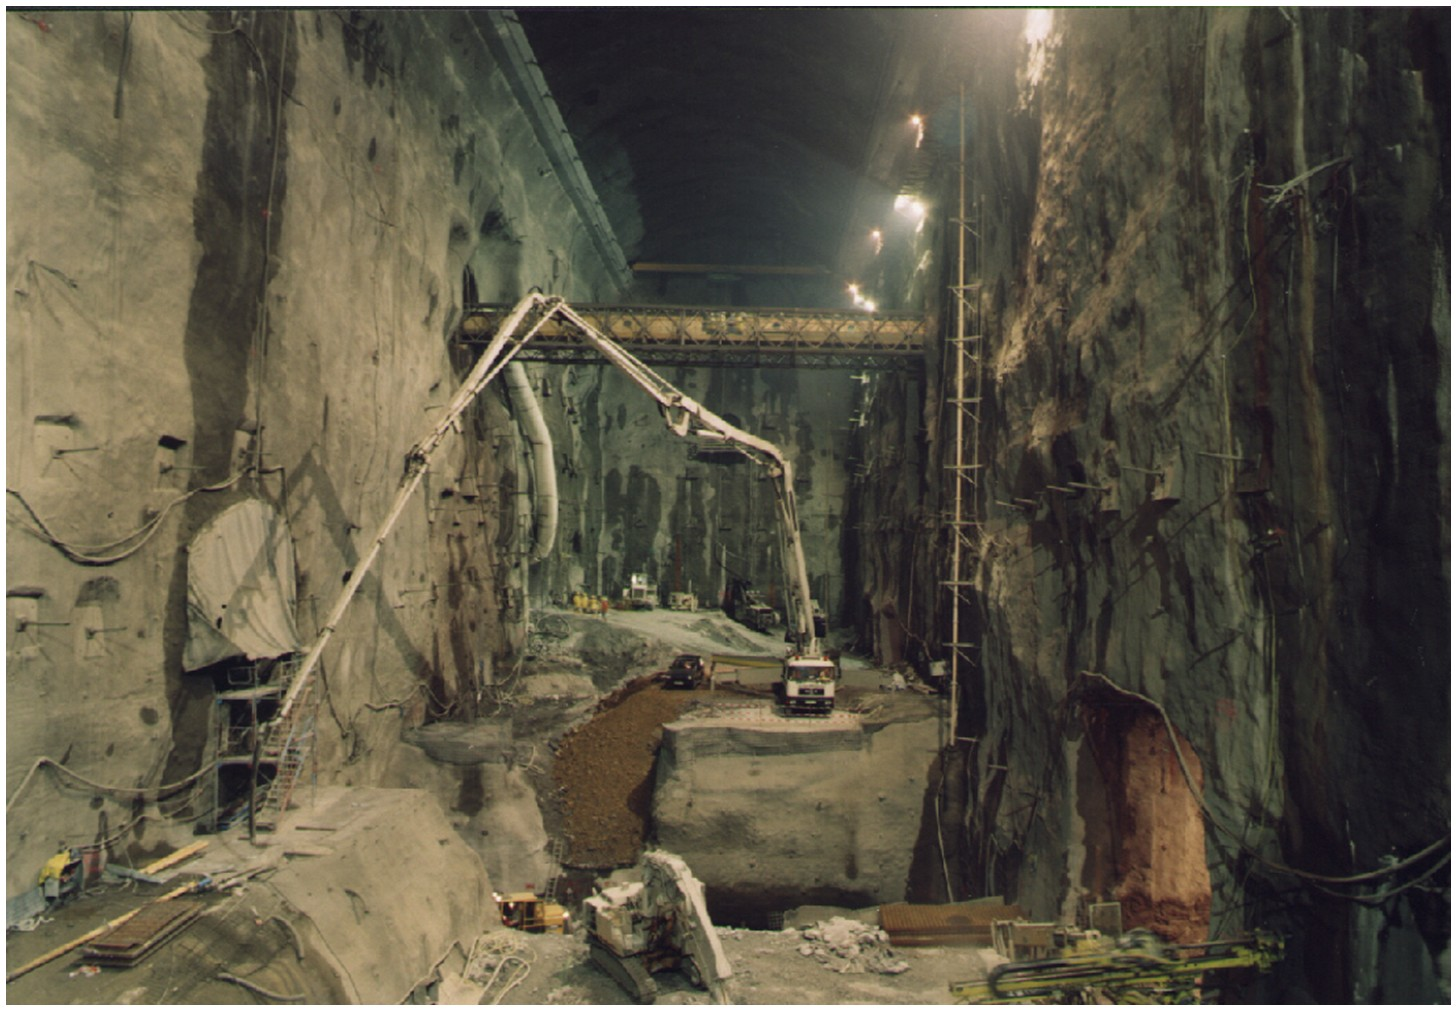
\includegraphics[width=12cm]{./Sec_SiteInfra/Figures/station.jpg}
\caption{The construction of the Robert Bourassa hydropower station in Quebec, Canada. 
Drill and blast was used to excavate the powerhouse with dimensions 296 m by
25 m by 47 m. More than 11,000 rock bolts were used.}
\label{fig:station}
\end{figure}
Einstein Telescope's caverns will be constructed by the drill and blast (D\&B) technique. 
Worldwide various such large underground
structures have been constructed. Fig.~\ref{fig:station} shows the underground
hydropower station in Quebec (Canada). 

\begin{figure}[htbp!]
\centering
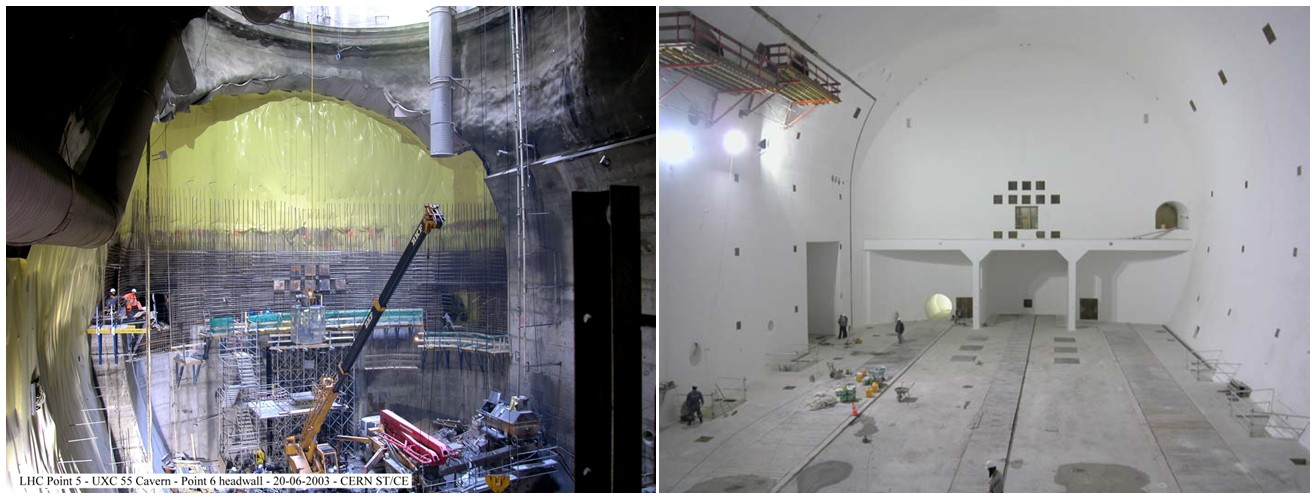
\includegraphics[width=16cm]{./Sec_SiteInfra/Figures/lhc.jpg}
\caption{The construction of the CMS cavern for the LHC project at CERN, Geneva.}
\label{fig:lhc}
\end{figure}
Einstein Telescope can profit from the large body of experience in underground cavern construction
for physics experiments. In particle physics there are LHC (previously LEP) at
CERN in Geneva, HERA at Desy in Hamburg, SLAC in Palo Alto and Fermilab in Chicago.
In addition, there are non-particle physics facilities as LNGS in Gran Sasso, LSM in Frejus, 
LSC in Canfranc, Kamioka in Japan and Dusel in South Dakota. 
Furthermore, there is experience from the mining industry.

As an example we show some of the experience in realizing large underground
caverns for the LHC project at CERN. These caverns host the Atlas and CMS experiments 
and have been constructed by D\&B. The left photo in Fig.~\ref{fig:lhc} shows the 
waterproofing foil used in the CMS
cavern at CERN. The right photo shows the completed cavern.
The Atlas cavern is located at a depth of 92\,m
and has a length of 55\,m, a width of 32\,m, and a height of 35\,m. The CMS
cavern is located at a depth of 20\,m and has a length, width and height of
53, 27, and 25\,m, respectively.

The construction of the Atlas cavern took 4.5 years and that of the CMS cavern 6.5 years. 
It is clear that for Einstein Telescope the various caverns must be constructed in parallel
in order to avoid excessive construction times.

\FloatBarrier
\subsubsection{Tunnels}
\label{subsec:tunnels}
The corner stations are connected by 10 km long tunnels. These tunnels have an inner diameter of 5.5 m and an outer diameter of 6.5 m (depending on geology and construction method). At the location of the cryolinks, the inner diameter will be increased to 6.0 m. The main caverns and the auxilliary caverns are connected by a double tunnel structure with a length of 300 m. Consequently, the observatory hosts more than 31 km of tunnel.
\begin{figure}[t!]
	\centering
	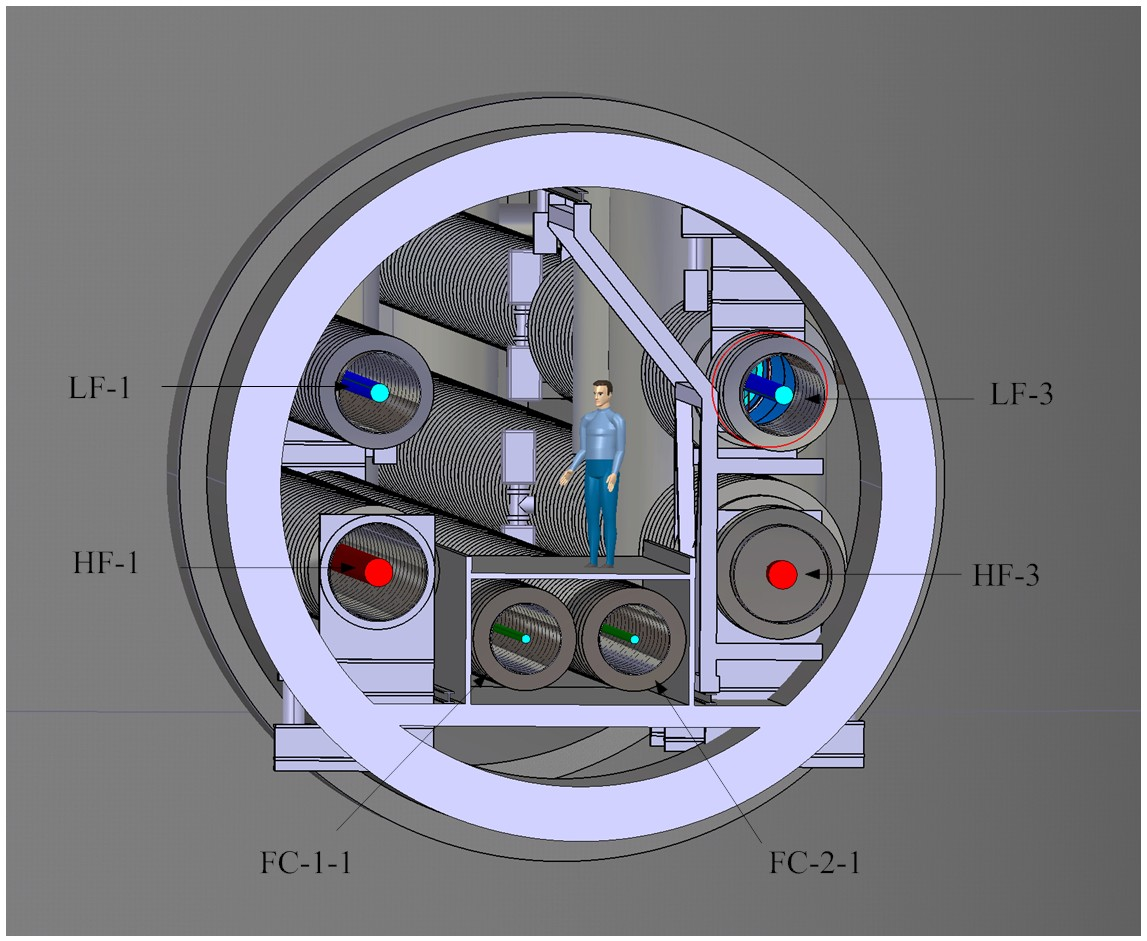
\includegraphics[width=12cm]{./Sec_SiteInfra/Figures/infra6.jpg}
	\caption{Schematic outline of the tunnel. The tunnel is occupied by the vacuum vessels that hold the low frequency (LF-1 and LF-2) and high frequency (HF-1 and HF-2) arms of two interferometers. In addition, the vacuum vessels for both filter (FC-1-1 and FC-2-1) cavities are housed. The inner diameter is 5.5 m and the tunnel wall has a thickness of 50 cm.}
	\label{fig:infra6}
\end{figure}

The main interferometer arm tunnels accommodate six vacuum beam pipes. In addition, the tunnel houses the services for electricity, water, compressed air, cryogenics, safety systems and air conditioning. The diameter of the tunnel is sufficiently large to allow transportation of vacuum beam pipes. An impression of the tunnel was shown in Fig.~\ref{fig:infra6}. During installation the tunnel will be equipped with a monorail system. This is used to transport the vacuum beam pipes. Provisions are made to accommodate the large vacuum valves in the tunnel walls, and to allow welding of the beam sections. For safety reasons the tunnel is divided into 500 m sections that are equipped with fire retarding doors, and safety shelters. The tunnel is equipped with an elaborate safety system that allows control of the airflow in order to direct the smoke in case of a fire.

\FloatBarrier
\subsubsection*{Tunnel construction}

At present there is a vast body of experience in tunnel construction.
This is to a large extent driven by the increasing worldwide demand 
for the creation of underground tunnels.
For the construction of high speed trains alone, in 2010
about 1000 km of lines is taken in operation, while the current demand
for 2020 is estimated at 3500 km \cite{itacet}.

\begin{figure}[htbp!]
\centering
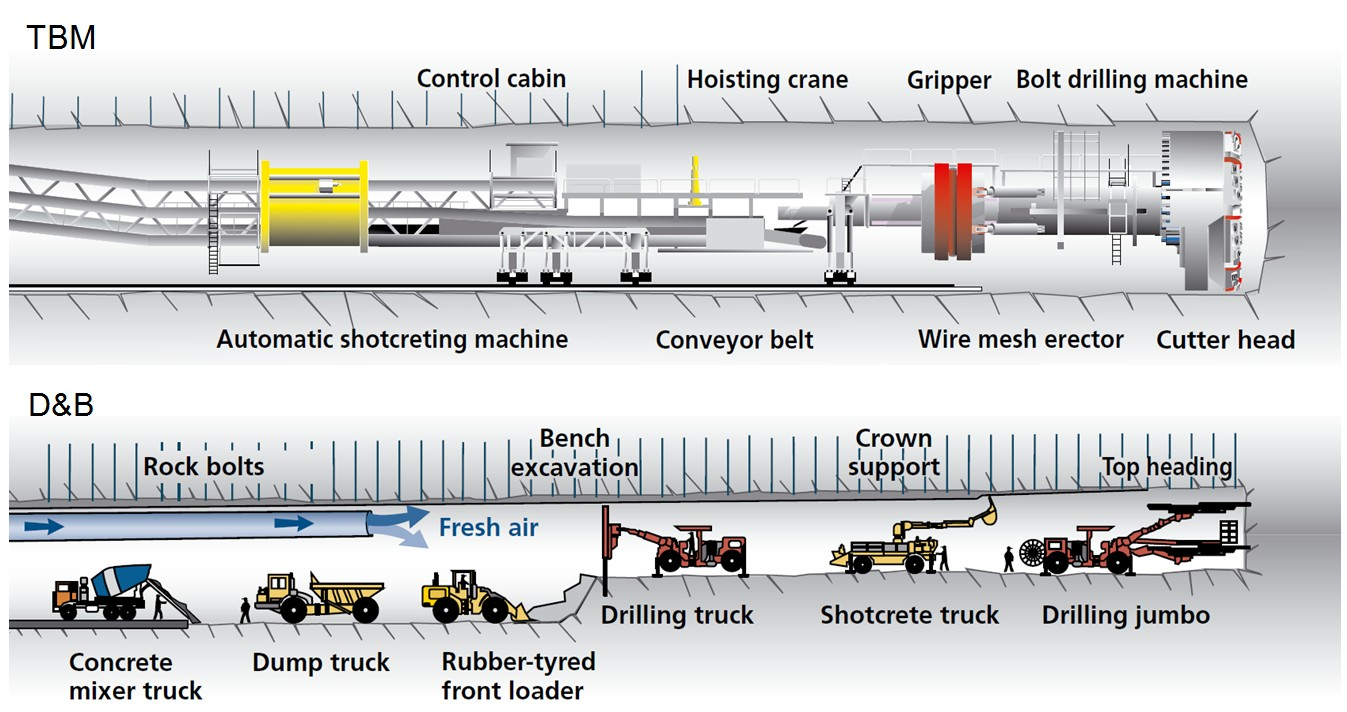
\includegraphics[width=16cm]{./Sec_SiteInfra/Figures/tunneling.jpg}
\caption{Underground tunnels can be constructed with tunnel boring machines (TBM),
or by using the conventional drill and blast method (D\&B).}
\label{fig:tunneling}
\end{figure}

For the construction of underground tunnels, two major technical
approaches can be distinguished: tunnel boring machines and
drill and blast. Fig.~\ref{fig:tunneling} schematically shows
the two techniques.

\FloatBarrier
\subsubsection*{Tunnel construction with TBMs}

The TBM technique is state of the art, and excavation rates of 20--25\,m per day
are routinely obtained. The geology must be well understood through site
surveys and one must realize that given the large size of the machine
(typically 400 m for the TBM and train combination) it is difficult to adapt to
changes (for example in geology). 

\begin{figure}[htbp!]
\centering
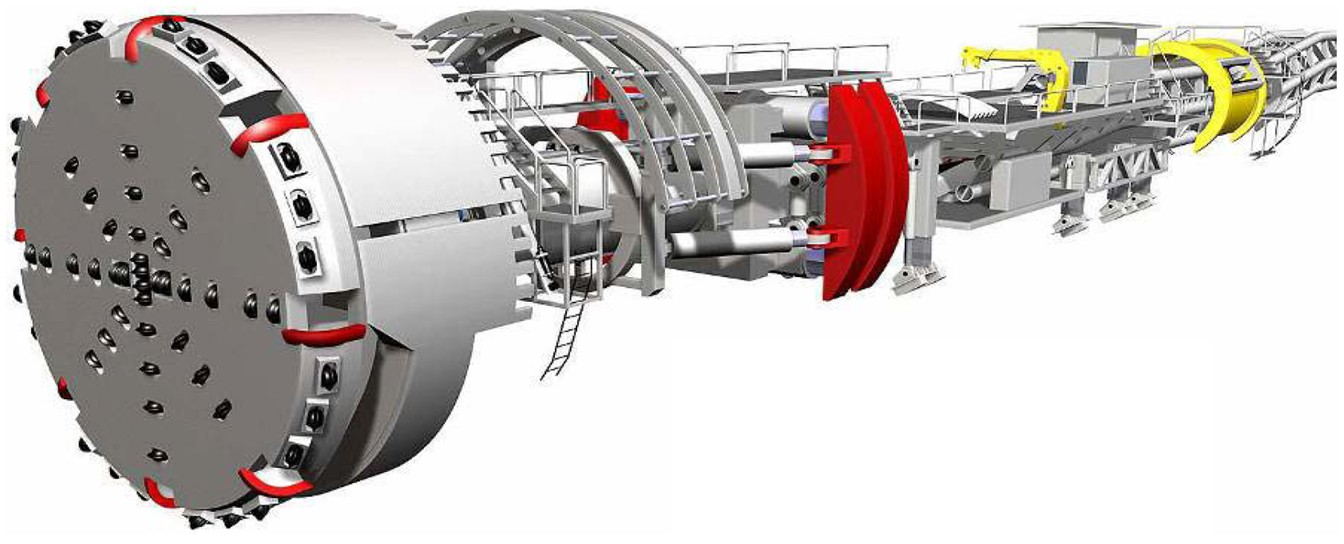
\includegraphics[width=14cm]{./Sec_SiteInfra/Figures/tbm.jpg}
\caption{Schematic representation of a gripper tunnel boring machine from Ref.~\cite{Herrenknecht}.}
\label{fig:tbm}
\end{figure}
Fig.~\ref{fig:tbm} shows an outline of a gripper TBM from Herrenknecht~\cite{Herrenknecht}.
This TBM has a 9.58\,m diameter and a length of 441\,m.  A power of 7.8\,MW is required
to drive the machine. The TBMs needed for Einstein Telescope would have a diameter of 6.5\,m.

The investment costs are large ($e.g.$ about 20\, M\euro for the TBM shown in Fig.~\ref{fig:tbm}) and set-up times are long. In the case of Einstein Telescope several TBMs would be required in order to  keep the construction time limited to 2 years. Sizeable diameters are needed for the vertical shafts in order to lower the equipment. A typical TBM cycle would involve boring 2 m of tunnel, followed by clearing out the rock. The tunnel wall support with anchors, shotcrete and steel arches is then implemented next. Tunnel construction would Per day shifts 1 and 2 would involve the above cycle, while shift 3 would be dedicated to the service and repair of the TBMs.

\FloatBarrier
\subsubsection*{Tunnel construction with D\&B}
 
The drill and blast technique is highly adaptable, but excavation rates are
limited to 6 - 10 m per day. A cycle consists of drill, charge, and detonate.
After ventilation, various tasks as support and muck removal take place. In good
rock conditions 1 cycle can be accomplished in an 8 hour shift.

\begin{figure}[htbp!]
\centering
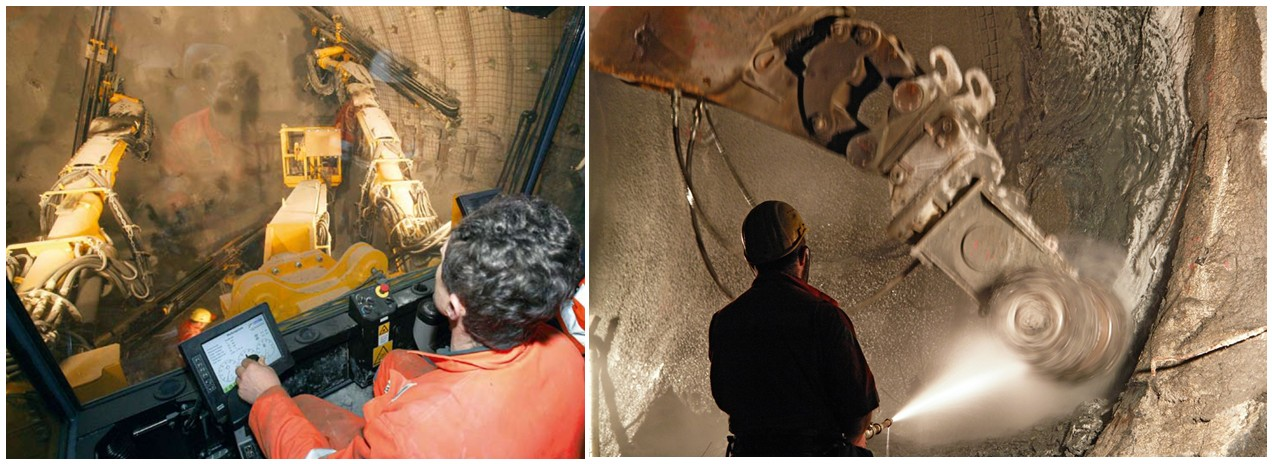
\includegraphics[width=16cm]{./Sec_SiteInfra/Figures/multihead.jpg}
\caption{Special tooling has been developed for the D\&B technique for tunneling.}
\label{fig:multihead}
\end{figure}
In order to cope with the relatively low advance rate, various teams
have to work in parallel. Advanced multi-head drilling tools have been
developed (see Fig.~\ref{fig:multihead}) in order to increase the advance rate.
\begin{figure}[htbp!]
\centering
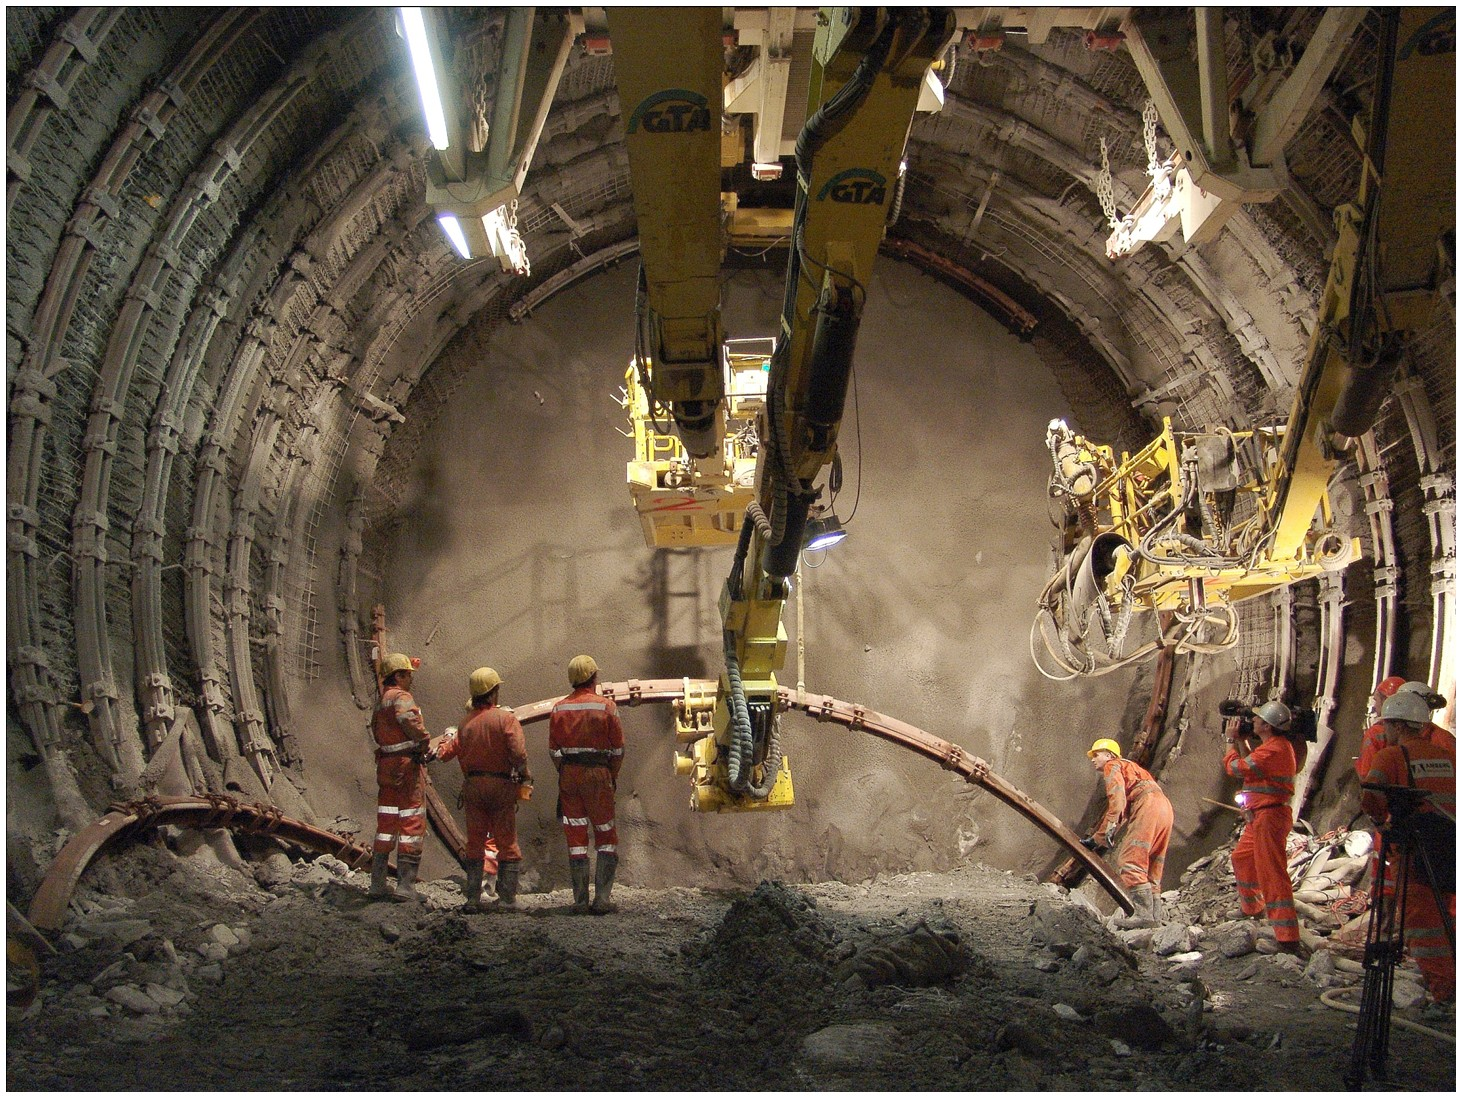
\includegraphics[width=10cm]{./Sec_SiteInfra/Figures/support.jpg}
\caption{Support of the tunnel walls can be erected in parallel to the drilling process.}
\label{fig:support}
\end{figure}
Fig.~\ref{fig:support} shows that support of the tunnel walls can be provided
in parallel with the multi-head drilling activities.

\FloatBarrier
\subsubsection*{Practical experience with tunnel construction}

There is a vast amount of experience available with tunnel construction
in various soil types and under various conditions. When long tunnels (typically with
lengths exceeding 6\,km) are considered and smooth walls are needed
($e.g.$ for high speed trains) then TBMs are often selected. Underground
infrastructure such as train tunnels are designed for a lifetime of about
100 years. Thus, special wall treatment is needed to ensure such a long lifetime.

\begin{figure}[htbp!]
\centering
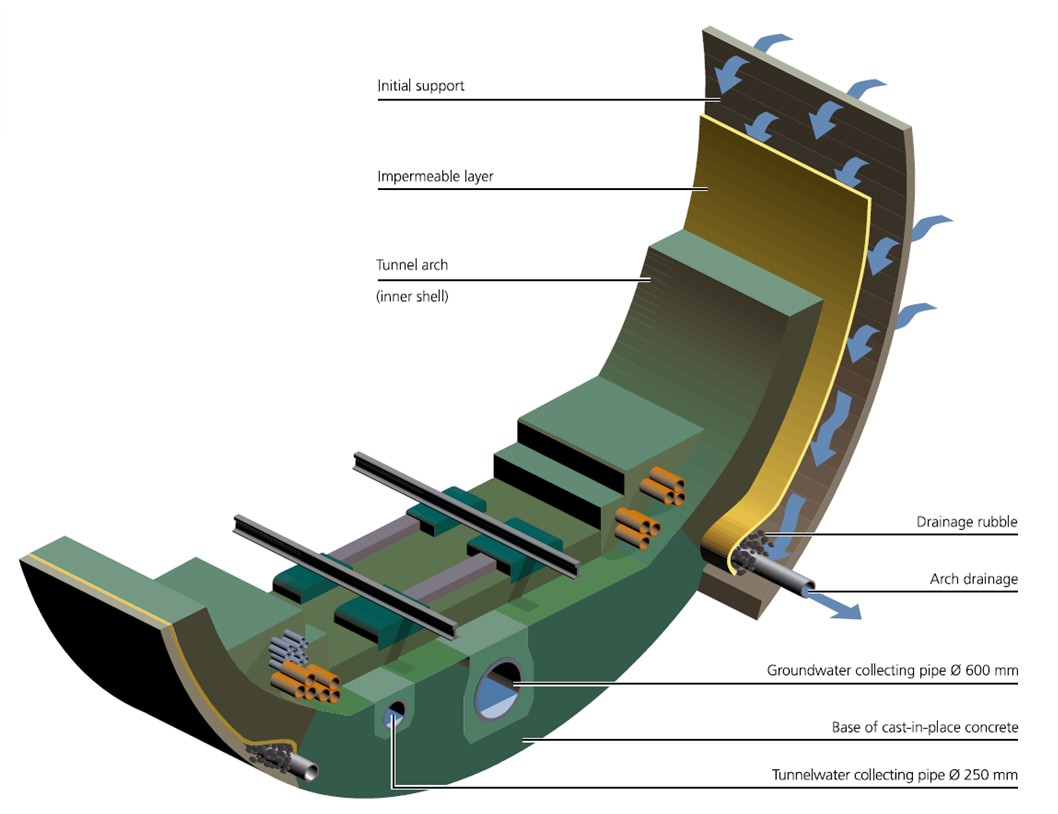
\includegraphics[width=11cm]{./Sec_SiteInfra/Figures/tunnelwall.jpg}
\caption{Wall segments used in the construction of the Gotthard-Basistunnel.
This project represents the world's largest underground construction.}
\label{fig:tunnelwall}
\end{figure}
Fig.~\ref{fig:tunnelwall} shows a wall segment that has been used in
the construction of the Gotthard-Basistunnel. The Gotthard-Basistunnel
represents the longest tunnel project in the world: a total tunnel length
of 98.135\,km has been constructed with TBM and 53.705\,km with D\&B. 
The lining is designed to handle corrosive water containing chloride,
sulphates, $etc.$ The impermeable layer avoids swelling of the concrete,
corrosion of the anchors, and sintering in the drainage system.
The drainage system is designed to prevent groundwater pressure buildup.

\begin{figure}[htbp!]
\centering
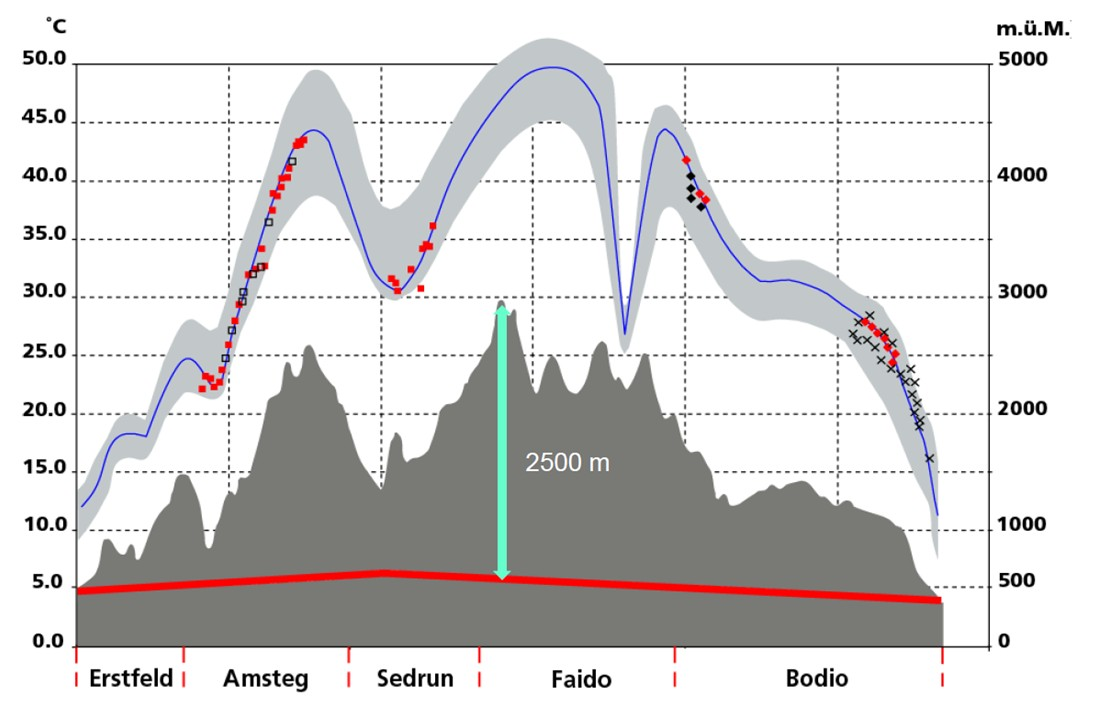
\includegraphics[width=14cm]{./Sec_SiteInfra/Figures/rocktemp.jpg}
\caption{Rock temperature distribution in the Gotthard-Basistunnel.
Temperature is shown on the left vertical axis and depth on the right axis
(m.\"u.M = meters above sea level). Erstfeld, Amsteg, $etc.$ are locations
along the tunnels.}
\label{fig:rocktemp}
\end{figure}
Construction of tunnels at large depth has various implications. Fig.~\ref{fig:rocktemp}
shows that in general rock temperature increases with depth. For train tunnels
these temperatures can be handled (since the trains act as pistons), but it may
cause troubles for Einstein Telescope. Sizeable and costly ventilation systems must be installed. These
systems also dilute dust and remove methane and radon (detection systems
for these gases must be installed). Other problems encountered in construction
at large depth include rockfall, rockbusts and possibly large deformations.

\begin{figure}[htbp!]
\centering
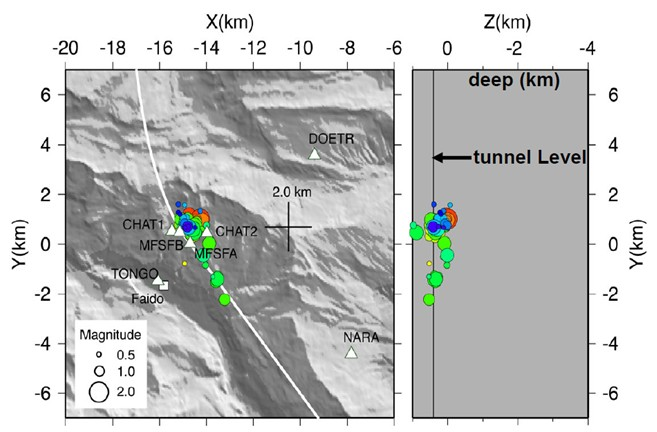
\includegraphics[width=12cm]{./Sec_SiteInfra/Figures/faido.jpg}
\caption{A seismic network set-up near Faido for the Gotthard-Basistunnel project
measured various micro tremors over a 2-year period.}
\label{fig:faido}
\end{figure}
For Einstein Telescope the issue of micro tremors may be significant. In the context of the
Gotthard-Basistunnel project, the Swiss Seismological Service, SED, recorded an
accumulation of seismic activity in the area of the MFS Faido (see Fig.~\ref{fig:faido}). 
Events were recorded in the period between March 2004 and June 2005. Normally, this
is a region with very low seismicity. A local seismic network was set-up at the 
multi-purpose station, MFS Faido, consisting of 9 stations at the surface, including one station from the
SDSNet. The stations were installed in a circular arrangement 10 to 15\,km
around the MFS Faido. In addition, 2 seismic stations were placed in the tunnel.
The hypocenters of the micro tremors were reconstruction in 3D. It was
clear that this seismicity was related to the underground tunnel construction.
The tremors were observed over at least a 2 year period.

\begin{figure}[htbp!]
\centering
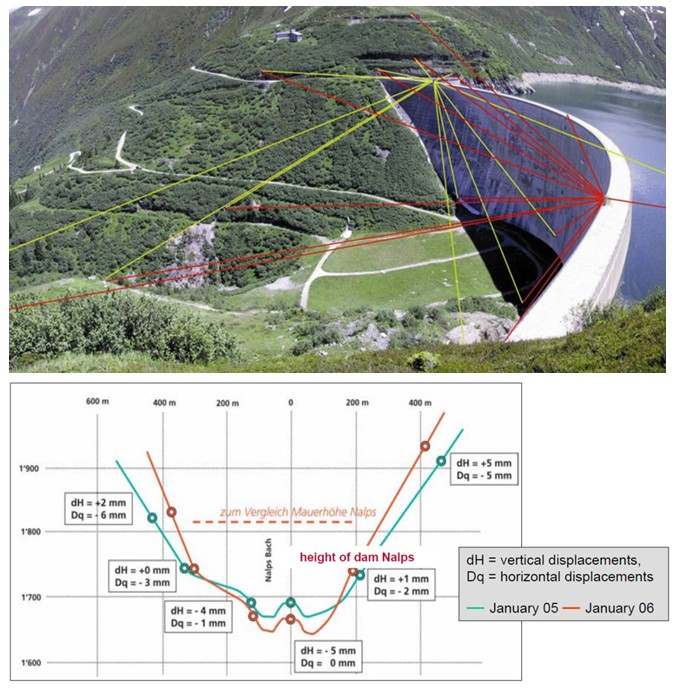
\includegraphics[width=12cm]{./Sec_SiteInfra/Figures/dam.jpg}
\caption{Horizontal and vertical displacements measured at the water dam Nalps
are related to the Gotthard-Basistunnel project.}
\label{fig:dam}
\end{figure}
Several water dams are located in the vicinity of the Gotthard-Basistunnel.
TPS and GPS measuring systems were installed around these dams in order
to monitor surface ground motion. Fig.~\ref{fig:dam} shows that several
mm displacements have been measured at these dams. The movements
are correlated with the TBM activity at Nalps North and were first observed
in December 2005. It is believed that although these dams are several km away
from the underground construction, the movements are due to changes induced
in the ground-water levels.

In general the construction of the Gotthard-Basistunnel went according to
expectations. However, a major problem occured in 2003 when crossing the horizontal
fault zone at Bodio. The TBM got stuck for more than 6 months and had to
be excavated. This was possible since the project features 2 tunnels (an
East and a West railway tube).

TBMs can also be used to drill tunnels in
soft soil. In that case special types of TBMs ($e.g.$ mixshield) must be used that have
a submerged wall, a working chamber, air cushion and pressure bulkhead. The
tunnel walls require advanced lining, while the TBM servicing requires special
manpower (divers). In general, tunnel construction in soft soil is considerably more expensive
than in hardrock.

The tunnel for the HERA ring (6.6\,km circumference) at DESY in Hamburg, Germany
and the LHC (the LEP) tunnel (26.7\,km circumference) at CERN in Geneva, Switzerland
have been constructed with TBMs. The 6 km tunnel for the LCGT project in the
Kamioka mountain in Japan will be constructed by D\&B. The Einstein Telescope team is in close
contact with LCGT and will more this project in detail over the next years.

\FloatBarrier
\subsubsection{Shafts}

Presently, it is not clear whether Einstein Telescope will have horizontal or vertical access.
In the case of vertical access, there is a significant increase in complexity of the
construction methods needed for shafts with depths exceeding 200\,m. 

In the following, we present a discussion that is based on vertical access, similar
to for example the LHC experiment at CERN (see Fig.~\ref{fig:shaft}).

\begin{figure}[htbp!]
\centering
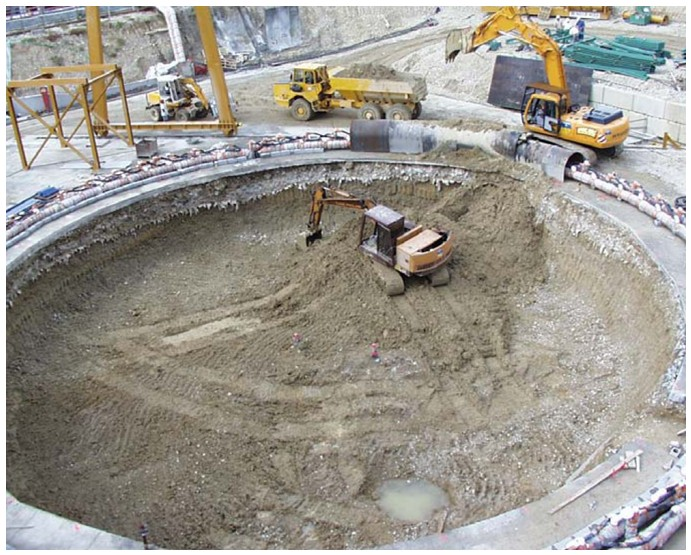
\includegraphics[width=12cm]{./Sec_SiteInfra/Figures/shaft.jpg}
\caption{The construction of the CMS access shaft for the LHC project at CERN, Geneva.
This shaft has an 18 m diameter and the entire CMS experiment was lowered through
it. To facility its construction, the ground at the shaft walls was frozen.}
\label{fig:shaft}
\end{figure}
Each corner station will be accessed through a 20 m diameter vertical shaft.
For excavation of the tunnels, the TBMs (in case this technique is adopted)
will be lowered through these shafts. After tunnel construction, the shafts
will be equipped with concrete elevator modules, staircases and will carry all
services (power, water, compressed air, ventilation ducts, $etc.$). Additional
shafts with a 10 m diameter are foreseen at the center of the arms.

\begin{figure}[htbp!]
\centering
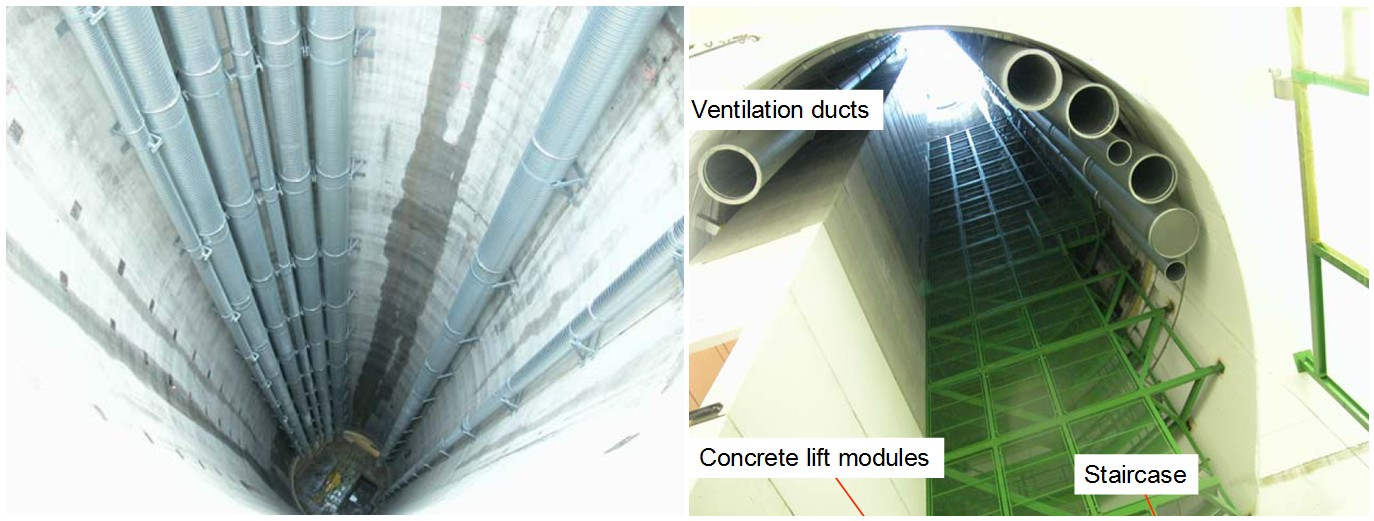
\includegraphics[width=16cm]{./Sec_SiteInfra/Figures/cmsshaft.jpg}
\caption{Completed access shafts for the LHC project at CERN, Geneva.}
\label{fig:cmsshaft}
\end{figure}
The top of the shafts will be integrated in large suface buildings. There
the equipment of the Einstein Telescope interferometers, such as the vacuum system, will
be prepared. Subsequently, the various modules will be lowered through the
shafts into the caverns using hoisting devices.

\FloatBarrier
\subsubsection{Final remarks}

Cost analysis shows that tunnels, shafts and caverns constitute the main cost drivers 
for the Einstein Telescope project. It is obvious that the cost of underground construction is site dependent
and contains large uncertainties at this stage of the project.

In follow up studies it is imperative that risk management of the project is assessed.
Worldwide many problems occured during underground construction. Furthermore,
in our discussions with insurance companies it became clear that part of the
risk cannot be insured ($e.g.$ water leaks in tunnels). The Technical Committee on
Geotechnical Reports of the Underground Technology Research Council has
established guidelines for a so-called geotechnical baseline report (GBR) for construction.
It is customary that a project starts by defining such a GBR in order to establish
a baseline on risks ($e.g.$ from geology) for industry and client. After
site selection such a GBR must be realized. It contains as much as possible detailed
site information based on geophysical surveys, lidar surveys, drilling samples,
probabilistic assessment of rock mass behavior, $etc.$ and requires close collaboration
between the client, industry, and geophysicists.

